% =====================================================================
% Laporan Tugas: Studi Ablasi RNN, LSTM, GRU vs ANN (Workshop Deep Learning, ITERA)
% FILE INI DIHASILKAN oleh scripts/bangun_laporan.py dari main.tex.tpl.
% Compile: latexmk -pdf main.tex   (atau unggah folder ini ke Overleaf)
% =====================================================================
\documentclass[conference,a4paper]{IEEEtran}
\IEEEoverridecommandlockouts

\usepackage[indonesian]{babel}
\usepackage[utf8]{inputenc}
\usepackage[T1]{fontenc}
\usepackage{cite}
\usepackage{amsmath,amssymb}
\usepackage{graphicx}
\usepackage{booktabs}
\usepackage{xcolor}
\usepackage[hidelinks]{hyperref}
\graphicspath{{gambar/}}

\begin{document}

\title{Studi Ablasi RNN, LSTM, dan GRU dibandingkan ANN untuk Prediksi Trafik Seluler Kota Milan}

\author{
\IEEEauthorblockN{Tobagus Ahmad Yogi}
\IEEEauthorblockA{NIM 124400075\\
Teknik Telekomunikasi,ITERA\\
Tobagus.124400075@student.itera.ac.id}
}

\maketitle

\begin{abstract}
Prediksi trafik per sel membantu operator mengalokasikan sumber daya jaringan. Laporan ini menguji apakah keunggulan model rekuren atas ANN pada prediksi aktivitas internet satu jam ke depan di kotak Duomo, Milan, bertahan ketika hyperparameter diubah. Dengan data per jam Telecom Italia, kami menjalankan studi ablasi satu faktor per waktu untuk lima faktor wajib (panjang jendela, ukuran \textit{hidden}, jumlah lapisan, \textit{learning rate}, kelompok fitur) dan dua faktor pilihan (\textit{batch size}, \textit{dropout}), masing-masing pada ANN, RNN, LSTM, dan GRU dengan tiga \textit{seed}. Pada konfigurasi acuan, RNN terbaik (test MAE 229,6 $\pm$ 5,1), disusul GRU, LSTM, dan ANN (309,9 $\pm$ 5,9), dan semuanya mengalahkan baseline naif terbaik (467,6). Faktor paling berpengaruh berbeda antar model: panjang jendela terutama merugikan ANN, sedangkan \textit{learning rate} $10^{-4}$ membuat semua model belum konvergen dalam 300 epoch. Menggabungkan nilai terbaik tiap faktor menurunkan val MAE ANN sebesar 14,5\,\% tetapi menaikkannya pada GRU (9,6\,\%), LSTM, dan RNN. Di Bandara Linate, urutan model acuan sama dengan di Duomo, tetapi konfigurasi terbaik hanya membantu ANN.
\end{abstract}

\begin{IEEEkeywords}
prediksi trafik seluler, RNN, LSTM, GRU, studi ablasi
\end{IEEEkeywords}

% ---------------------------------------------------------------------
\section{Pendahuluan}
Operator seluler meramal trafik per sel untuk mengatur kapasitas dan menghemat energi. Model sekuensial seperti RNN, LSTM \cite{hochreiter1997lstm}, dan GRU \cite{cho2014gru} lazim dipakai karena membaca data secara berurutan dengan jumlah parameter yang tidak bergantung pada panjang jendela, sedangkan ANN harus meratakan seluruh jendela menjadi satu vektor. Di Sesi 2 workshop, keempat model dibandingkan dengan \emph{satu} konfigurasi, dan hasilnya RNN $\approx$ GRU $<$ LSTM $<$ ANN pada test MAE. Pertanyaan laporan ini: apakah kesimpulan itu tetap berlaku bila hyperparameter diubah?

Studi ablasi mengubah satu faktor dalam satu waktu dari konfigurasi acuan dan mengamati dampaknya, sehingga pengaruh tiap faktor dapat dipisahkan. Kontribusi laporan ini: (1) ablasi tujuh faktor pada empat model dengan tiga \textit{seed} di kotak Duomo; (2) pemilihan konfigurasi terbaik per model berdasarkan val MAE, bukan test MAE, dengan pelaporan di minggu test dan minggu Natal; dan (3) uji generalisasi di Bandara Linate.

% ---------------------------------------------------------------------
\section{Data dan Metode}

\subsection{Dataset}
Data berasal dari Telecom Italia Big Data Challenge \cite{barlacchi2015milan} dalam versi agregat per jam dari \cite{zhang2021fedda}, 4 November--29 Desember 2013. Setiap jam memuat aktivitas internet (\texttt{net}, target), panggilan (\texttt{call}), dan SMS (\texttt{sms}); ditambah jam dan hari dalam pekan yang dikodekan sin--cos, sehingga ada tujuh fitur. Lokasi utama adalah kotak Duomo (5060), dan lokasi kelompok adalah kode 5, Bandara Linate (kotak 4489), sesuai digit terakhir NIM 124400075. Gambar~\ref{fig:pola} memperlihatkan perbedaan keduanya: rata-rata \texttt{net} per jam pada periode latih adalah 3376,4 di Duomo dan 86,0 di Linate.

\begin{figure}[t]
  \centering
  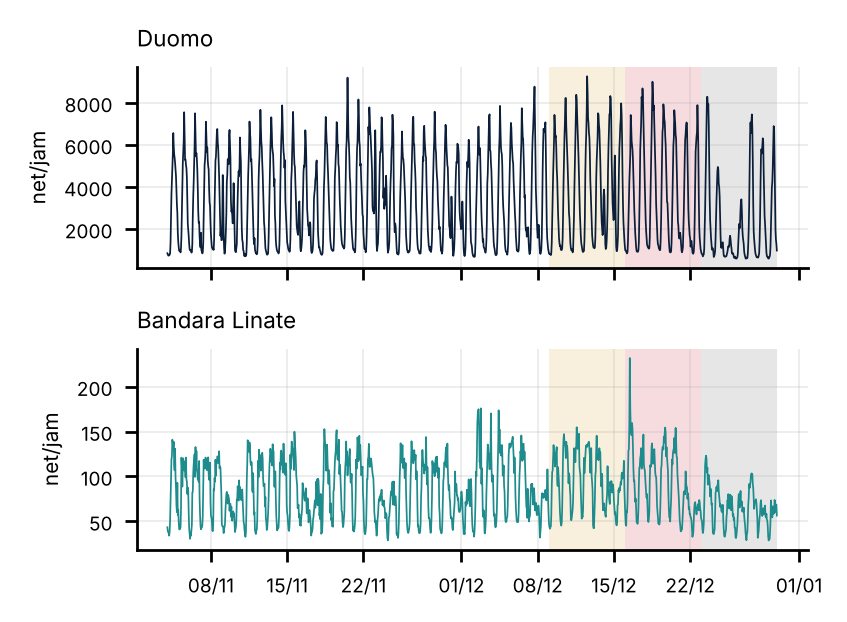
\includegraphics[width=\linewidth]{fig_pola.png}
  \caption{Aktivitas internet per jam di Duomo dan Bandara Linate. Bidang berwarna: minggu validasi (kuning), test (merah), dan Natal (abu-abu). Di Linate, trafik minggu Natal turun dan mendatar.}
  \label{fig:pola}
\end{figure}

\subsection{Pembagian Data dan Praproses}
Pembagian murni berdasarkan waktu: latih 11 November--8 Desember (672 jam), validasi 9--15 Desember, test 16--22 Desember, dan Natal 23--29 Desember. Data deret waktu tidak boleh diacak karena jam-jam bertetangga sangat berkorelasi, sehingga pengacakan akan membocorkan masa depan ke data latih. Standardisasi memakai rata-rata dan simpangan baku sebelum minggu validasi. Model menerima jendela $W$ jam terakhir dan meramal \texttt{net} satu jam berikutnya.

\subsection{Model dan Konfigurasi Acuan}
ANN meratakan jendela $[W, 7]$ menjadi satu vektor lalu melewatkannya ke lapisan padat ber-ReLU. RNN, LSTM, dan GRU memproses jendela langkah demi langkah, dan keluaran langkah terakhir masuk ke lapisan linear. Konfigurasi acuan mengikuti Sesi 2: $W=24$, horizon 1 jam, \textit{hidden} ANN 32, RNN 68, LSTM 33, GRU 38 (jumlah parameter sengaja dibuat mirip, 5.305--6.497), ANN 2 lapisan dan model rekuren 1 lapisan, ketujuh fitur, Adam dengan \textit{learning rate} $10^{-3}$ \cite{kingma2015adam}, \textit{batch size} 64, tanpa \textit{dropout}, loss MSE, serta \textit{early stopping} dengan \textit{patience} 30 dan maksimum 300 epoch (bobot dengan val loss terendah dipakai). Implementasi memakai PyTorch \cite{paszke2019pytorch}.

\subsection{Protokol Ablasi dan Evaluasi}
Faktor yang diubah satu per satu: A1 panjang jendela $W\in\{6,12,24,48,168\}$; A2 ukuran \textit{hidden} $\{16,32,64,128\}$; A3 jumlah lapisan $\{1,2,3\}$; A4 \textit{learning rate} $\{10^{-4},10^{-3},10^{-2}\}$; A5 kelompok fitur $\{$\texttt{net}, \texttt{net+call+sms}, \texttt{net+waktu}, semua$\}$; B1 \textit{batch size} $\{16,64,256\}$; B2 \textit{dropout} $\{0;0{,}2;0{,}5\}$. Hipotesis B1 dan B2 dituliskan \emph{sebelum} eksperimen dijalankan. Setiap konfigurasi dilatih dengan \textit{seed} 0, 1, 2, dan hasil dilaporkan sebagai rata-rata $\pm$ simpangan baku sampel. Metrik adalah MAE, RMSE, dan MAPE pada skala asli. Ablasi dinilai dengan \textbf{val MAE}; minggu test dan Natal hanya dipakai untuk acuan, konfigurasi terbaik, dan uji generalisasi. Konfigurasi terbaik tiap model dibentuk dengan mengambil, untuk setiap faktor, nilai dengan val MAE rata-rata terendah, lalu menggabungkannya. Seluruh pelatihan dijalankan di Google Colab (GPU T4, PyTorch 2.11.0+cu130): 273 pelatihan unik (348 baris pada \texttt{ablasi.csv}, 75 di antaranya disalin karena konfigurasinya identik) dengan total waktu 17,7 menit.

% ---------------------------------------------------------------------
\section{Hasil}

\subsection{Baseline Naif dan Acuan (Bagian 0)}
Tabel~\ref{tab:base} memuat tiga baseline naif dan konfigurasi acuan di Duomo. Pada minggu test, urutan model sama dengan Sesi 2: RNN (229,6 $\pm$ 5,1) $\approx$ GRU (237,2 $\pm$ 9,3) $<$ LSTM (273,6 $\pm$ 25,4) $<$ ANN (309,9 $\pm$ 5,9). Selisih RNN dan GRU lebih kecil daripada simpangan baku GRU, sehingga keduanya tidak dapat dibedakan. Semua model mengalahkan baseline naif terbaik pada minggu test (467,6, \emph{minggu lalu}); RNN memangkas galat 50,9\,\% dari baseline itu. Pada minggu Natal, baseline terbaik adalah \emph{nilai terakhir} (431,2) dan hanya RNN (421,2 $\pm$ 2,4) yang berada di bawahnya, tipis; ANN (680,1) dan LSTM (586,0) jauh di atasnya. Pola Natal berbeda dari empat minggu latih (rata-rata trafik turun 35,3\,\% dibanding minggu test), sehingga model yang hanya melihat pekan biasa tidak siap menghadapinya, sedangkan baseline nilai terakhir menyesuaikan diri seketika.

\begin{table}[t]
  \centering
  \caption{Baseline naif dan konfigurasi acuan di Duomo, horizon 1 jam. MAE rata-rata $\pm$ simpangan baku (3 \textit{seed}); baseline naif tanpa simpangan baku.}
  \label{tab:base}
  \footnotesize
  \setlength{\tabcolsep}{3pt}
  \begin{tabular}{@{}lrccc@{}}
    \toprule
    Model & Param & val MAE & test MAE & natal MAE \\
    \midrule
    Naif: nilai terakhir & --- & 662,6 & 600,9 & 431,2 \\
    Naif: kemarin & --- & 595,3 & 552,2 & 921,5 \\
    Naif: minggu lalu & --- & 492,8 & 467,6 & 1426,2 \\
    \midrule
    ANN & 6.497 & 248,9 $\pm$ 8,9 & 309,9 $\pm$ 5,9 & 680,1 $\pm$ 52,0 \\
    RNN & 5.305 & 206,1 $\pm$ 7,4 & \textbf{229,6 $\pm$ 5,1} & 421,2 $\pm$ 2,4 \\
    LSTM & 5.578 & 230,5 $\pm$ 12,2 & 273,6 $\pm$ 25,4 & 586,0 $\pm$ 56,8 \\
    GRU & 5.397 & 207,5 $\pm$ 3,8 & 237,2 $\pm$ 9,3 & 468,2 $\pm$ 21,8 \\
    \bottomrule
  \end{tabular}
\end{table}

\subsection{Ablasi Wajib (A1--A5)}
Gambar~\ref{fig:abl} merangkum val MAE seluruh faktor.

\begin{figure*}[t]
  \centering
  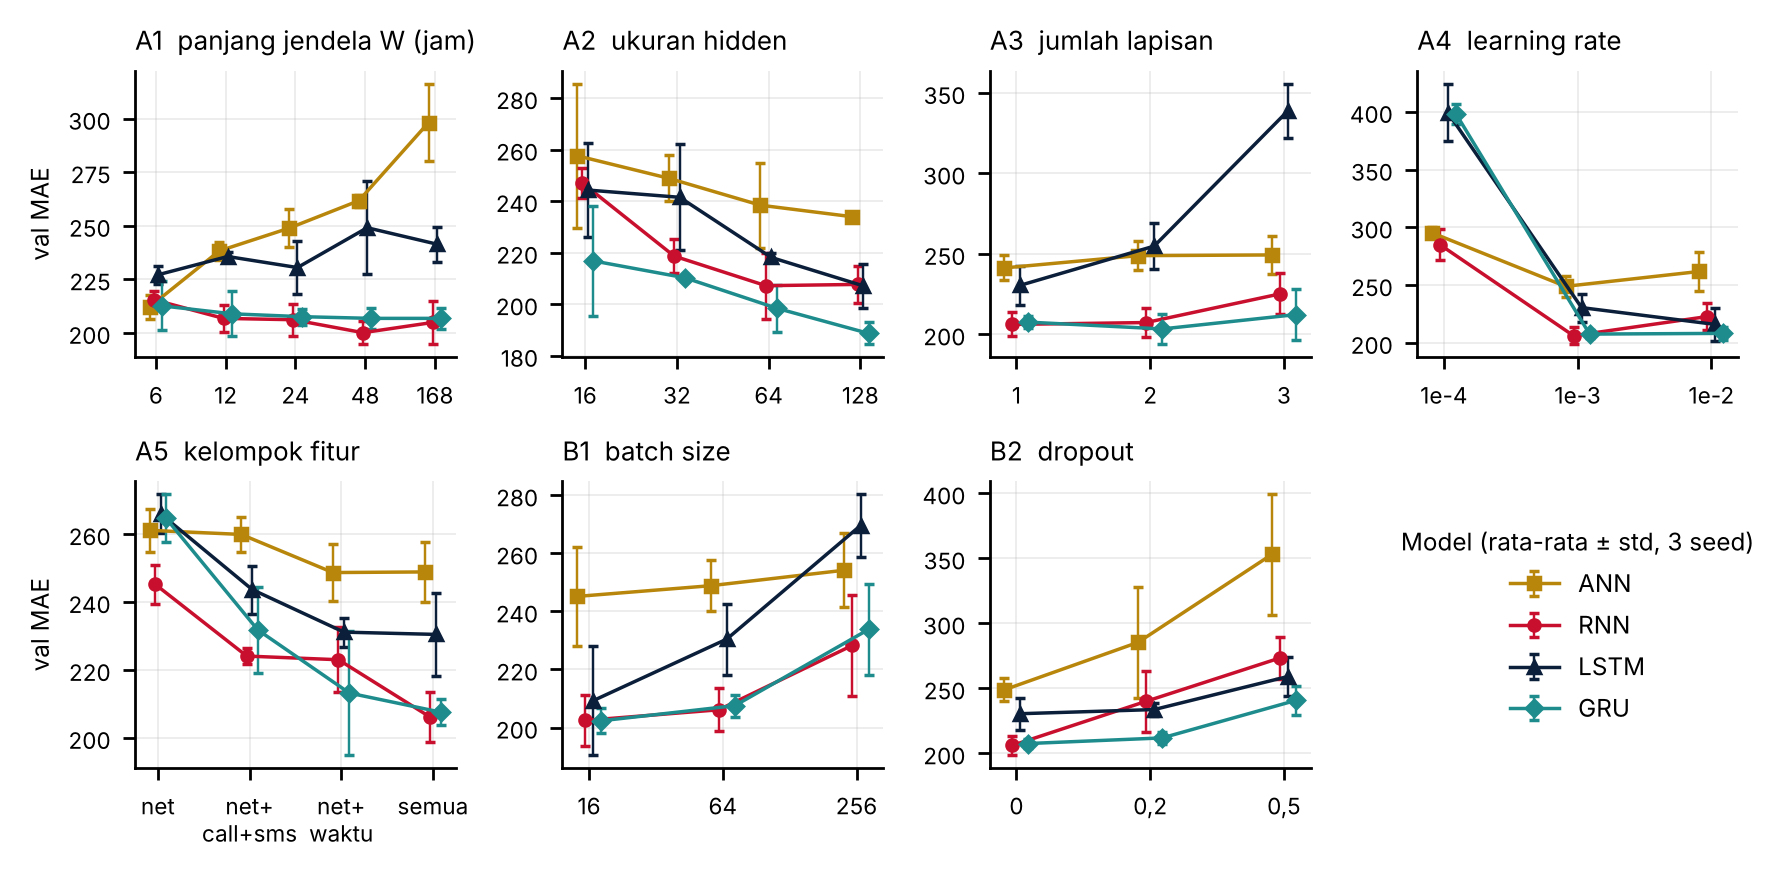
\includegraphics[width=0.93\textwidth]{fig_ablasi.png}
  \caption{Val MAE (rata-rata $\pm$ simpangan baku, 3 \textit{seed}) terhadap tiap faktor ablasi di Duomo. Panel A1--A5 adalah faktor wajib, B1--B2 faktor pilihan. Sumbu-$y$ berbeda tiap panel.}
  \label{fig:abl}
\end{figure*}

\textbf{A1, panjang jendela.} Val MAE ANN naik monoton dari 212,1 ($W=6$) ke 298,2 ($W=168$), kenaikan 40,6\,\%, sementara parameternya membengkak dari 2.465 menjadi 38.753 (15,7$\times$). Model rekuren hampir datar (RNN 200,1--215,5, GRU 206,7--212,6) dengan parameter tetap, 5,3--5,6 ribu. Jendela yang lebih panjang tidak selalu lebih baik; ia terutama merugikan ANN. Pada $W=6$, ANN (212,1) setara dengan GRU (212,6) dan RNN (215,5).

\textbf{A2, ukuran \textit{hidden}.} Model yang lebih besar membantu keempat model sampai 128 tanpa tanda \textit{overfitting} pada val MAE, mungkin karena \textit{early stopping} membatasi kapasitas efektif. GRU turun dari 216,8 ke 188,7 dan menjadi yang terbaik di grid; RNN jenuh pada 64 (207,2 vs 207,7 pada 128). Perbandingan ini tidak setara dari sisi parameter: pada \textit{hidden} 128, LSTM memiliki 70.273 parameter, 4,0$\times$ RNN (17.665).

\textbf{A3, jumlah lapisan.} Menumpuk lapisan umumnya tidak membantu. LSTM paling sensitif: 230,5 (1 lapisan) menjadi 338,9 (3 lapisan), kenaikan 47,0\,\%. RNN naik ke 225,1 pada 3 lapisan, dan ANN hampir tidak berubah (241,2--249,3). Hanya GRU sedikit membaik pada 2 lapisan (203,3 vs 207,5), selisih yang berada dalam simpangan baku. Model lebih dalam berhenti lebih cepat: epoch RNN turun dari 164 ke 96.

\textbf{A4, \textit{learning rate}.} Pada $10^{-4}$ semua model di semua \textit{seed} berhenti di batas 300 epoch dan val MAE tinggi (285,0--399,4): pelatihan belum konvergen. Pada $10^{-2}$ pelatihan jauh lebih cepat (62--68 epoch) dengan hasil setara $10^{-3}$ untuk GRU (208,2 vs 207,5), lebih baik untuk LSTM (215,9 vs 230,5), dan lebih buruk untuk RNN (222,7 vs 206,1) dan ANN (261,8 vs 248,9); simpangan baku antar \textit{seed} naik pada keempat model.

\textbf{A5, kelompok fitur.} Hanya \texttt{net} adalah yang terburuk di semua model (245,2--266,0). Dari \texttt{net} ke semua fitur, val MAE turun 16,0\,\% (RNN), 21,6\,\% (GRU), 13,4\,\% (LSTM), dan hanya 4,7\,\% (ANN). Fitur waktu memberi manfaat lebih besar daripada \texttt{call}+\texttt{sms} untuk ANN, LSTM, dan GRU; pada RNN keduanya setara dan saling melengkapi (223,0 $\rightarrow$ 206,1 bila digabung). Ketiga model rekuren memperoleh manfaat fitur lebih besar daripada ANN.

\subsection{Ablasi Pilihan (B1--B2)}
Tabel~\ref{tab:hip} menguji hipotesis yang ditulis sebelum eksperimen terhadap val MAE Gambar~\ref{fig:abl}.

\begin{table*}[t]
  \centering
  \caption{Hipotesis Bagian B (ditulis sebelum eksperimen) dan hasilnya terhadap val MAE di Duomo.}
  \label{tab:hip}
  \footnotesize
  \renewcommand{\arraystretch}{1.15}
  \begin{tabular}{@{}p{0.27\textwidth}p{0.45\textwidth}p{0.22\textwidth}@{}}
    \toprule
    Hipotesis & Bukti & Status \\
    \midrule
    B1: \textit{batch} 256 paling buruk di keempat model & Val 256 vs 64: ANN 254,2 vs 248,9; RNN 228,3 vs 206,1; LSTM 269,6 vs 230,5; GRU 233,8 vs 207,5 (GRU 3/3 \textit{seed} berhenti di 300 epoch) & Terbukti \\
    B1: \textit{batch} 16 dan 64 berselisih lebih kecil dari simpangan baku & Selisih val 16 vs 64: ANN 3,7, RNN 3,7, GRU 5,2, LSTM 21,2 (LSTM 209,2 vs 230,5) & Sebagian: ANN, RNN ya; GRU, LSTM tidak \\
    B1: urutan model tidak berubah & Pada 16: RNN 202,4 $\approx$ GRU 202,3 $<$ LSTM 209,2 $<$ ANN 245,2. Pada 256: LSTM 269,6 lebih buruk dari ANN 254,2 & Sebagian: berubah pada 256 \\
    B2: \textit{dropout} 0,2 membantu ANN, netral untuk rekuren & Val 0,2 vs 0: ANN 285,4 vs 248,9; RNN 240,0 vs 206,1; LSTM 233,7 vs 230,5; GRU 211,9 vs 207,5 & Tidak terbukti: ANN dan RNN memburuk \\
    B2: \textit{dropout} 0,5 memperburuk semua model & Val 0,5 vs 0: ANN 353,0 vs 248,9; RNN 273,3 vs 206,1; LSTM 259,1 vs 230,5; GRU 240,7 vs 207,5 & Terbukti \\
    B2: \textit{dropout} kurang berpengaruh daripada $W$ dan fitur & Selisih val maks.--min.: \textit{dropout} vs $W$ vs fitur: ANN 104,1/86,1/12,4; RNN 67,2/15,4/39,1; LSTM 28,6/22,0/35,5; GRU 33,2/5,8/57,1 & Tidak terbukti: lebih berpengaruh dari $W$ di semua model, dari fitur di ANN dan RNN \\
    \bottomrule
  \end{tabular}
\end{table*}

\textit{Batch size} 256 terbukti merugikan semua model, dan GRU berhenti di batas 300 epoch pada ketiga \textit{seed} karena hanya sekitar tiga pembaruan per epoch. \textit{Batch} 16 berguna terutama untuk LSTM. \textit{Dropout} tidak membantu model mana pun: ANN dan RNN memburuk sejak 0,2, dan 0,5 memperburuk semua. Dugaan kami, \textit{dropout} di sini dipasang pada keluaran lapisan terakhir (atau tiap lapisan tersembunyi ANN), tempat seluruh informasi untuk meramal satu nilai kontinu dikompresi, sehingga menjatuhkan unit langsung menambah galat ramalan; kami tidak menguji dugaan ini.

\subsection{Konfigurasi Terbaik (Bagian C)}
Hasil seleksi val MAE tertera di Tabel~\ref{tab:cd} (blok Duomo). Perubahan dari acuan: ANN $W=6$, \textit{hidden} 128, 1 lapisan, fitur \texttt{net+waktu}, \textit{batch} 16; RNN $W=48$, \textit{batch} 16; LSTM $W=6$, \textit{hidden} 128, \textit{learning rate} $10^{-2}$, \textit{batch} 16; GRU $W=48$, \textit{hidden} 128, 2 lapisan, \textit{batch} 16. Pada ANN, nilai \texttt{net+waktu} hanya unggul 0,2 poin dari semua fitur, jauh di bawah simpangan baku; aturan val MAE tetap diterapkan apa adanya.

Penggabungan ini \textbf{tidak menurunkan val MAE untuk tiga dari empat model}: ANN turun 14,5\,\% (248,9 $\rightarrow$ 212,7), tetapi RNN naik 1,6\,\%, LSTM 4,5\,\%, dan GRU 9,6\,\% (207,5 $\rightarrow$ 227,4). Pada minggu test, keempat model lebih rendah dari acuan: ANN 9,9\,\%, LSTM 9,6\,\%, GRU 2,9\,\%, RNN 1,4\,\%, tetapi hanya perbaikan ANN dan LSTM yang melampaui simpangan baku; perbaikan GRU dan RNN berada di dalamnya. Pada minggu Natal, semua model membaik (ANN 17,3\,\%, LSTM 20,9\,\%, GRU 5,6\,\%, RNN 8,5\,\%), dan RNN (385,4 $\pm$ 13,8) semakin jauh di bawah baseline nilai terakhir (431,2). Urutan model pada test tetap RNN 226,3 $\approx$ GRU 230,2 $<$ LSTM 247,3 $<$ ANN 279,2.

\subsection{Uji Generalisasi (Bagian D)}
Konfigurasi acuan dan terbaik dari Duomo dilatih ulang tanpa perubahan di Bandara Linate (Tabel~\ref{tab:cd}, blok Linate). Urutan model acuan sama dengan di Duomo: RNN (7,5 $\pm$ 0,1) $\approx$ GRU (7,5 $\pm$ 0,2) $<$ LSTM (8,2 $\pm$ 0,2) $<$ ANN (8,8 $\pm$ 0,7), dan semuanya mengalahkan baseline naif terbaik (10,1, \emph{nilai terakhir}). Konfigurasi terbaik \textbf{tidak ikut membaik} di sini: hanya ANN yang turun (10,2\,\%), sedangkan GRU (+2,0\,\%), LSTM (+4,1\,\%), dan RNN (+13,0\,\%) bergeser naik; selisih GRU dan RNN masih di dalam simpangan baku (RNN 1,1), sedangkan LSTM sedikit di luarnya. Urutan model pun berubah: ANN (7,9) kini mengungguli LSTM (8,5) dan RNN (8,5). Val MAE justru turun untuk ANN, GRU, dan LSTM (mis.\ GRU 9,2 $\rightarrow$ 8,3), jadi perbaikan pada val tidak berpindah ke minggu test. Pada minggu Natal, \emph{semua} model, baik acuan (10,8--14,4) maupun terbaik, kalah dari baseline nilai terakhir (7,1).

\begin{table*}[t]
  \centering
  \caption{Konfigurasi acuan (a) dan terbaik (t) pada Duomo (Bagian C) dan Bandara Linate (Bagian D, konfigurasi dari Duomo tanpa diubah). MAE rata-rata $\pm$ simpangan baku, 3 \textit{seed}. ``hid'' = \textit{hidden}, ``lap.'' = lapisan, bs = \textit{batch size}. Parameter konfigurasi terbaik: ANN 4.097, RNN 5.305, LSTM 70.273, GRU 151.809.}
  \label{tab:cd}
  \footnotesize
  \setlength{\tabcolsep}{3pt}
  \begin{tabular}{@{}ll cc cc cc@{}}
    \toprule
    & Perubahan dari acuan & \multicolumn{2}{c}{val MAE} & \multicolumn{2}{c}{test MAE} & \multicolumn{2}{c}{natal MAE} \\
    \cmidrule(lr){3-4}\cmidrule(lr){5-6}\cmidrule(lr){7-8}
    Model & (konfigurasi t) & a & t & a & t & a & t \\
    \midrule
    \multicolumn{8}{@{}l}{\textit{Duomo (kotak 5060)}} \\
    ANN & $W{=}6$, hid 128, 1 lap., \texttt{net+waktu}, bs 16 & 248,9 $\pm$ 8,9 & 212,7 $\pm$ 5,4 & 309,9 $\pm$ 5,9 & 279,2 $\pm$ 13,4 & 680,1 $\pm$ 52,0 & 562,7 $\pm$ 29,8 \\
    RNN & $W{=}48$, bs 16 & 206,1 $\pm$ 7,4 & 209,5 $\pm$ 3,2 & 229,6 $\pm$ 5,1 & 226,3 $\pm$ 4,9 & 421,2 $\pm$ 2,4 & 385,4 $\pm$ 13,8 \\
    LSTM & $W{=}6$, hid 128, lr $10^{-2}$, bs 16 & 230,5 $\pm$ 12,2 & 240,9 $\pm$ 5,1 & 273,6 $\pm$ 25,4 & 247,3 $\pm$ 12,8 & 586,0 $\pm$ 56,8 & 463,4 $\pm$ 5,3 \\
    GRU & $W{=}48$, hid 128, 2 lap., bs 16 & 207,5 $\pm$ 3,8 & 227,4 $\pm$ 7,3 & 237,2 $\pm$ 9,3 & 230,2 $\pm$ 8,5 & 468,2 $\pm$ 21,8 & 442,1 $\pm$ 26,9 \\
    Naif terbaik & & \multicolumn{2}{c}{492,8 (minggu lalu)} & \multicolumn{2}{c}{467,6 (minggu lalu)} & \multicolumn{2}{c}{431,2 (nilai terakhir)} \\
    \midrule
    \multicolumn{8}{@{}l}{\textit{Bandara Linate (kotak 4489)}} \\
    ANN & $W{=}6$, hid 128, 1 lap., \texttt{net+waktu}, bs 16 & 8,7 $\pm$ 0,0 & 8,4 $\pm$ 0,2 & 8,8 $\pm$ 0,7 & 7,9 $\pm$ 0,5 & 14,4 $\pm$ 0,5 & 14,0 $\pm$ 1,7 \\
    RNN & $W{=}48$, bs 16 & 8,5 $\pm$ 0,1 & 8,5 $\pm$ 0,2 & 7,5 $\pm$ 0,1 & 8,5 $\pm$ 1,1 & 10,8 $\pm$ 0,1 & 11,1 $\pm$ 0,8 \\
    LSTM & $W{=}6$, hid 128, lr $10^{-2}$, bs 16 & 9,3 $\pm$ 0,1 & 8,4 $\pm$ 0,1 & 8,2 $\pm$ 0,2 & 8,5 $\pm$ 0,2 & 12,8 $\pm$ 0,8 & 13,5 $\pm$ 0,6 \\
    GRU & $W{=}48$, hid 128, 2 lap., bs 16 & 9,2 $\pm$ 0,1 & 8,3 $\pm$ 0,2 & 7,5 $\pm$ 0,2 & 7,7 $\pm$ 0,5 & 11,4 $\pm$ 0,9 & 11,6 $\pm$ 0,6 \\
    Naif terbaik & & \multicolumn{2}{c}{10,4 (nilai terakhir)} & \multicolumn{2}{c}{10,1 (nilai terakhir)} & \multicolumn{2}{c}{7,1 (nilai terakhir)} \\
    \bottomrule
  \end{tabular}
\end{table*}

\begin{figure*}[t]
  \centering
  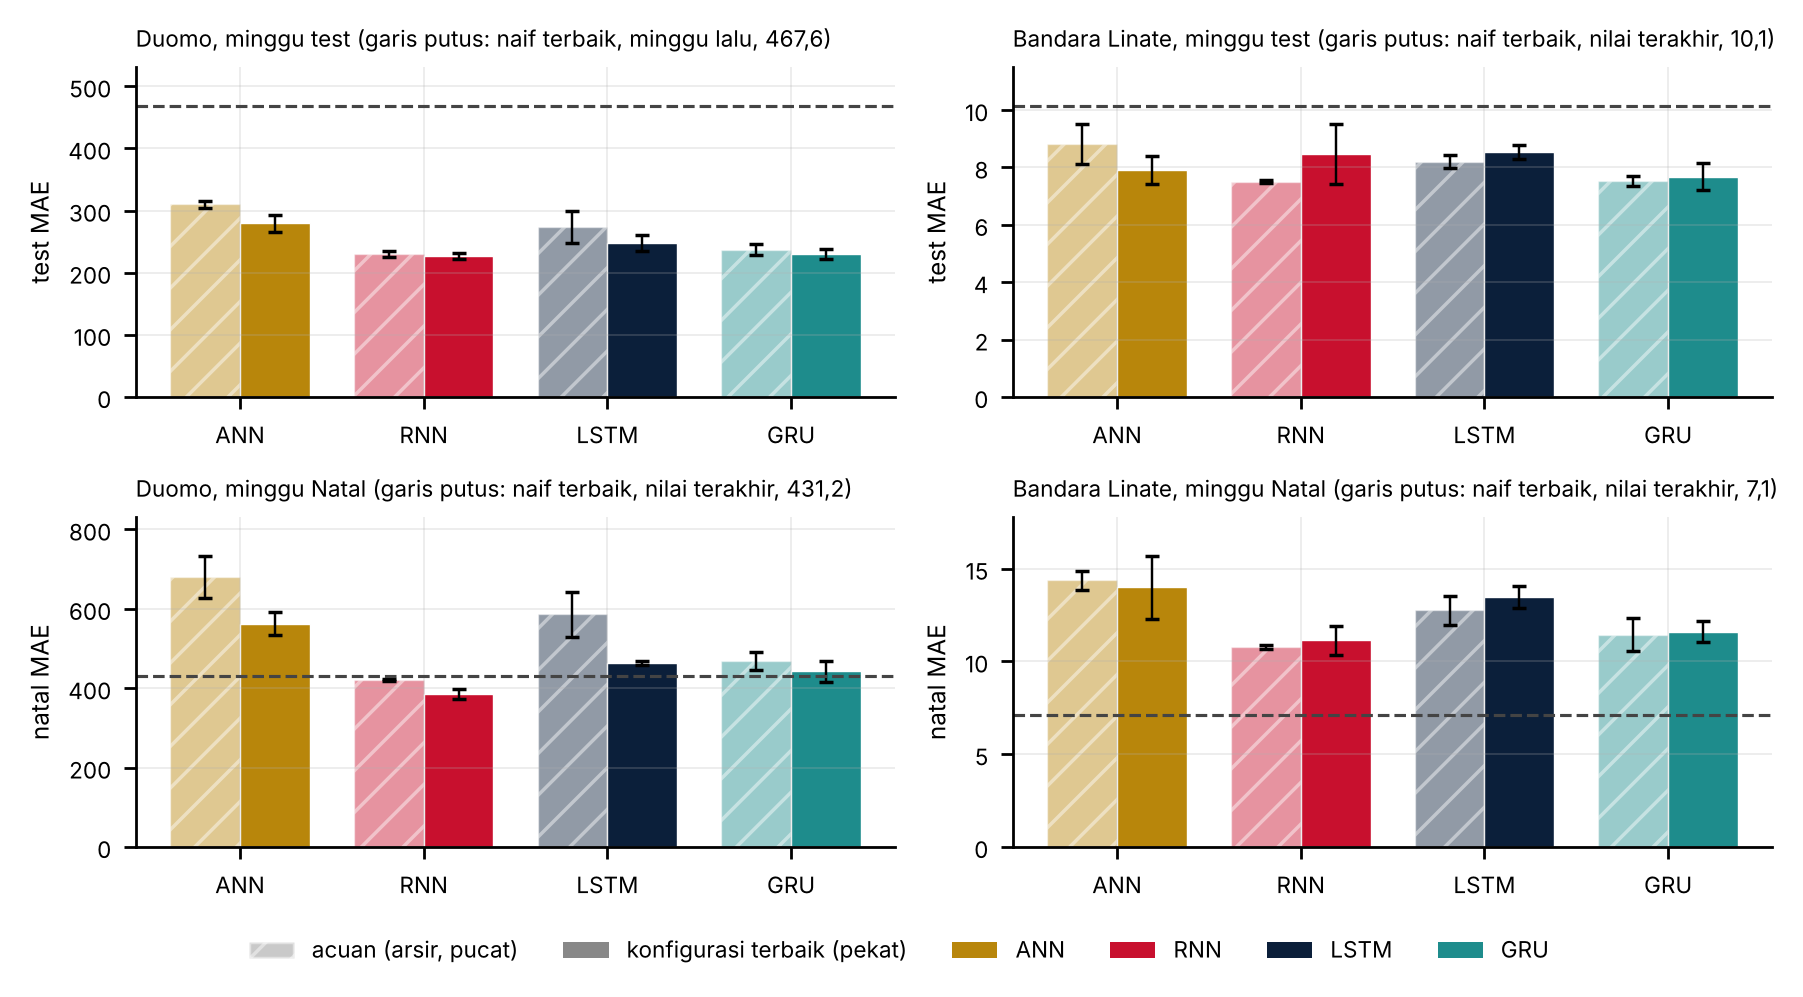
\includegraphics[width=0.86\textwidth]{fig_CD.png}
  \caption{Test MAE dan Natal MAE, konfigurasi acuan (arsir) dan terbaik (pekat), di Duomo dan Bandara Linate (rata-rata $\pm$ simpangan baku, 3 \textit{seed}). Garis putus: baseline naif terbaik pada split yang sama.}
  \label{fig:cd}
\end{figure*}

% ---------------------------------------------------------------------
\section{Pembahasan}
\textbf{Apakah keunggulan model rekuren bertahan?} Sebagian. Urutan RNN $\approx$ GRU $<$ LSTM $<$ ANN bertahan pada konfigurasi acuan di Duomo dan Linate, pada konfigurasi terbaik di Duomo, dan pada \textit{batch} 16 dan 64, tetapi bukan hukum umum: ia berubah pada konfigurasi terbaik di Linate (ANN 7,9 di bawah LSTM dan RNN, keduanya 8,5). Pada $W=6$, ANN setara dengan model rekuren (val MAE 212,1 vs 212,6 pada GRU); pada \textit{hidden} 128, GRU (188,7) mengungguli RNN (207,7); dan pada \textit{batch} 256, LSTM (269,6) lebih buruk daripada ANN (254,2). Keunggulan rekuren dengan demikian terutama berasal dari kemampuannya membaca jendela panjang tanpa menambah parameter: kerugian ANN pada $W$ besar (A1) adalah efek terbesar kedua pada ANN setelah \textit{dropout}. Di antara model rekuren, RNN paling sederhana dan pada sebagian besar konfigurasi tidak kalah dari LSTM dan GRU. Dugaan kami, pada hanya 672 sampel latih dan dependensi yang pendek (pola harian, $W=24$), gerbang LSTM dan GRU belum diperlukan; ini tidak diuji langsung.

\textbf{Faktor paling berpengaruh.} Menurut selisih val MAE terbesar antar nilai faktor, \textit{learning rate} paling dominan pada ketiga model rekuren (RNN 78,9 hingga GRU 190,9), tetapi hampir seluruhnya berasal dari nilai $10^{-4}$ yang belum konvergen dalam 300 epoch. Pada ANN, \textit{dropout} (104,1) dan $W$ (86,1) lebih berpengaruh daripada \textit{learning rate} (46,4). Faktor berikutnya bergantung model: jumlah lapisan pada LSTM (108,4) dan fitur pada GRU (57,1). Panjang jendela hampir tidak berpengaruh pada GRU (5,8). Karena pengaruhnya bergantung model, kesimpulan dari satu konfigurasi acuan tidak dapat dipindahkan begitu saja.

\textbf{Mengapa gabungan terbaik justru bisa lebih buruk?} Ablasi satu faktor mengasumsikan pengaruh yang aditif, padahal faktor saling berinteraksi. Pada GRU, \textit{hidden} 128 dan 2 lapisan bersama-sama menghasilkan 151.809 parameter, 28$\times$ konfigurasi acuan (5.397) untuk 672 sampel latih; pelatihan berhenti pada rata-rata 61 epoch, dan val MAE memburuk. LSTM serupa (70.273 parameter, 13$\times$). Di sisi lain, test dan Natal MAE membaik pada kedua model itu. Dengan satu minggu validasi dan satu minggu test, kami tidak dapat memastikan mana yang menggambarkan generalisasi sebenarnya; yang dapat dikatakan adalah bahwa val MAE saja bukan penuntun yang andal untuk konfigurasi gabungan. Seleksi terhadap banyak pilihan pada satu minggu validasi yang sama dengan \textit{early stopping} juga cenderung memberi val MAE yang terlalu optimistis: ANN, yang paling banyak berubah, menunjukkan selisih terbesar antara val (212,7) dan test (279,2).

\textbf{Mengapa Linate berbeda?} Trafik Linate berukuran jauh lebih kecil (rata-rata 86,0 vs 3376,4) sehingga MAE tidak dapat dibandingkan langsung (RNN: 8,2\,\% dari rata-rata minggu test di Linate, 6,3\,\% di Duomo). Pola harian Linate lebih lemah dan selisih akhir pekan--hari kerja lebih tajam: autokorelasi lag 24 jam hanya 0,74 (Duomo 0,91), dan rasio rata-rata akhir pekan terhadap hari kerja 0,72 (Duomo 0,97). Konfigurasi terbaik dari Duomo kemungkinan disesuaikan dengan pola harian yang tajam di sana, sehingga tidak otomatis cocok untuk lokasi yang polanya lebih berisik; kami tidak menguji penjelasan ini. Pada minggu Natal, rata-rata trafik Linate turun 29,5\,\% dibanding minggu test dan tampak mendatar (Gambar~\ref{fig:pola}), sehingga baseline nilai terakhir (7,1) sulit dikalahkan oleh model yang dilatih pada pekan biasa.

\textbf{Keterbatasan.} Hanya satu pembagian waktu dengan empat minggu latih; validasi dan test masing-masing satu minggu; simpangan baku diambil dari tiga \textit{seed} sehingga kasar dan tidak disertai uji signifikansi; ablasi satu faktor tidak mengukur interaksi; horizon hanya satu jam; dan hanya dua lokasi. Minggu Natal berada di luar distribusi latih, sehingga hasilnya menguji ketahanan, bukan kualitas ramalan biasa.

% ---------------------------------------------------------------------
\section{Kesimpulan}
Pada prediksi trafik satu jam ke depan di Duomo, urutan RNN $\approx$ GRU $<$ LSTM $<$ ANN bertahan di konfigurasi acuan dan terbaik (test MAE terbaik: RNN 226,3 $\pm$ 4,9; ANN 279,2 $\pm$ 13,4), tetapi tidak di setiap konfigurasi: ANN menyusul model rekuren pada jendela pendek ($W=6$). \textit{Learning rate} yang terlalu kecil adalah kesalahan paling mahal, sedangkan \textit{dropout} dan \textit{batch} 256 merugikan. Menggabungkan nilai terbaik tiap faktor hanya menurunkan val MAE ANN (14,5\,\%) dan menaikkannya pada GRU (9,6\,\%), LSTM, dan RNN, meski test dan Natal MAE membaik. Di Bandara Linate, urutan model acuan sama tetapi konfigurasi terbaik hanya menguntungkan ANN, dan pada minggu Natal baseline nilai terakhir mengalahkan semua model. Pesan praktisnya: hasil ablasi perlu divalidasi ulang per lokasi, dan konfigurasi gabungan harus diuji, bukan diasumsikan.

% ---------------------------------------------------------------------
\section*{Kontribusi Anggota}
\begin{tabular}{@{}lp{0.62\linewidth}@{}}
  Tobagus Ahmad Yogi & Seluruh pekerjaan (kelompok satu orang): menjalankan eksperimen di Google Colab, pemilihan konfigurasi, dan penyusunan laporan. \\
\end{tabular}

\section*{Pernyataan Penggunaan AI}
Claude (Anthropic) dipakai untuk membantu memahami petunjuk tugas dan memandu pengaturan Google Colab, menyusun draf hipotesis B1--B2 sebelum eksperimen dijalankan, memilih konfigurasi terbaik secara mekanis dari \texttt{ablasi.csv} berdasarkan val MAE, menulis skrip analisis \texttt{scripts/analisis.py}, serta menyusun draf laporan ini. Seluruh pelatihan model dijalankan oleh penulis dengan \texttt{tugas\_ablasi.ipynb}, dan setiap angka dalam laporan dihasilkan skrip tersebut dari \texttt{hasil/ablasi.csv}.

\section*{Kode dan Data}
Kode, notebook beserta output, dan seluruh hasil run tersedia di \url{https://github.com/tobaylegendsavaga-create/dlw-tugas-ra-124400075}.

\bibliographystyle{IEEEtran}
\bibliography{references}

\end{document}
